\section*{Modelisation of the system}
    The system is composed of a vehicle that will drag a sledge that transports a magnetometer. The towing vehicle is a tank type vehicle, and the sled is attached to it with a rope. Assuming that the rope is constantly under tension, we are able to find the equations describing the dynamics of the system. By noting $x$ the state of the system and $u$ its inputs, the dynamics of the system is described by :

    \begin{empheq}[left={\dot{x} = f(x, u) =}\empheqlbrace]{align}
        \dot{x_1} &=\ \dfrac{u_1 + u_2}{2}.cos(x_3) \label{eq:x}\\
        \dot{x_2} &=\ \dfrac{u_1 + u_2}{2}.sin(x_3) \label{eq:y}\\
        \dot{x_3} &=\ u_2 - u_1 \label{eq:theta}\\
        \dot{x_4} &=\ - \dfrac{u_1 + u_2}{2}.sin(x_4) - \dot{x_3} \label{eq:phi}
    \end{empheq}

    Here $x_1$, $x_2$ and $x_3$ are respectively the abscissa, the ordinate and the heading of the trailing robot, $x_4$ is the angle of the sled to the tractor vehicle.

    \begin{figure}[!htb]
        \centering
        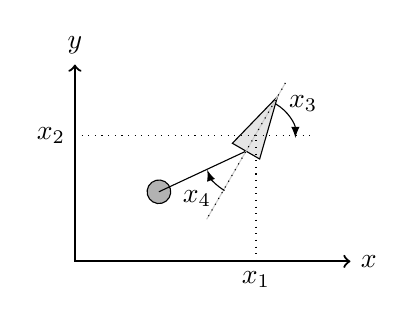
\begin{tikzpicture}
            \draw [<->,thick] (0,2.5) node (yaxis) [above] {$y$}
                |- (3.5,0) node (xaxis) [right] {$x$};

            \tikzset{
                robot/.pic = {
                    \draw[black,fill=gray!20] (0,0) -- (0.2,0.8) -- (0.4,0) -- cycle;
                    \draw[black,fill=gray!60] (0.2,0) -- (-0.5,-1) circle(0.15);
                    \draw[gray!40] (0.2,-1) -- (0.2,1);
                    \draw[dotted] (0.2,1) -- (0.2,-1);

                }
            }
            \pic[rotate=-30] at (2, 1.5) {robot};
            \draw[dotted] (0,1.6) node (x2) [left] {$x_2$} -- (2.3,1.6) -- (2.3,0) node (x1) [below] {$x_1$};
            
            \draw[dotted] (2.3,1.6) -- (3,1.6);
            \draw[>=latex, ->] (2.55,2) arc (60:0:0.5);
            \draw node at (2.9,2) {$x_3$};
            \draw[>=latex, ->] (1.9,0.9) arc (240:200:0.5);
            \draw node at (1.55,0.8) {$x_4$};

        \end{tikzpicture}
    \end{figure}